% !TeX spellcheck = de_DE
\section{Methodology}
\label{sec:methodology}
	
	\subsection{Measured Data}
	\label{ssec:measured-data}
	
		As a ...
		The reflectance $\varrho(\lambda)$ of a sample at a wavelength $\lambda \in \Lambda$ is recorded as
		\[
			-\lg \varrho(\lambda) = -\frac{\ln \varrho(\lambda)}{\ln 10}
		\]
		Figure \ref{fig:soil-spec-rnd} shows six randomly chosen soil spectra in a diagram.
		\begin{figure*}
			\centering
			% GNUPLOT: LaTeX picture with Postscript
\begingroup
  \makeatletter
  \providecommand\color[2][]{%
    \GenericError{(gnuplot) \space\space\space\@spaces}{%
      Package color not loaded in conjunction with
      terminal option `colourtext'%
    }{See the gnuplot documentation for explanation.%
    }{Either use 'blacktext' in gnuplot or load the package
      color.sty in LaTeX.}%
    \renewcommand\color[2][]{}%
  }%
  \providecommand\includegraphics[2][]{%
    \GenericError{(gnuplot) \space\space\space\@spaces}{%
      Package graphicx or graphics not loaded%
    }{See the gnuplot documentation for explanation.%
    }{The gnuplot epslatex terminal needs graphicx.sty or graphics.sty.}%
    \renewcommand\includegraphics[2][]{}%
  }%
  \providecommand\rotatebox[2]{#2}%
  \@ifundefined{ifGPcolor}{%
    \newif\ifGPcolor
    \GPcolorfalse
  }{}%
  \@ifundefined{ifGPblacktext}{%
    \newif\ifGPblacktext
    \GPblacktexttrue
  }{}%
  % define a \g@addto@macro without @ in the name:
  \let\gplgaddtomacro\g@addto@macro
  % define empty templates for all commands taking text:
  \gdef\gplbacktext{}%
  \gdef\gplfronttext{}%
  \makeatother
  \ifGPblacktext
    % no textcolor at all
    \def\colorrgb#1{}%
    \def\colorgray#1{}%
  \else
    % gray or color?
    \ifGPcolor
      \def\colorrgb#1{\color[rgb]{#1}}%
      \def\colorgray#1{\color[gray]{#1}}%
      \expandafter\def\csname LTw\endcsname{\color{white}}%
      \expandafter\def\csname LTb\endcsname{\color{black}}%
      \expandafter\def\csname LTa\endcsname{\color{black}}%
      \expandafter\def\csname LT0\endcsname{\color[rgb]{1,0,0}}%
      \expandafter\def\csname LT1\endcsname{\color[rgb]{0,1,0}}%
      \expandafter\def\csname LT2\endcsname{\color[rgb]{0,0,1}}%
      \expandafter\def\csname LT3\endcsname{\color[rgb]{1,0,1}}%
      \expandafter\def\csname LT4\endcsname{\color[rgb]{0,1,1}}%
      \expandafter\def\csname LT5\endcsname{\color[rgb]{1,1,0}}%
      \expandafter\def\csname LT6\endcsname{\color[rgb]{0,0,0}}%
      \expandafter\def\csname LT7\endcsname{\color[rgb]{1,0.3,0}}%
      \expandafter\def\csname LT8\endcsname{\color[rgb]{0.5,0.5,0.5}}%
    \else
      % gray
      \def\colorrgb#1{\color{black}}%
      \def\colorgray#1{\color[gray]{#1}}%
      \expandafter\def\csname LTw\endcsname{\color{white}}%
      \expandafter\def\csname LTb\endcsname{\color{black}}%
      \expandafter\def\csname LTa\endcsname{\color{black}}%
      \expandafter\def\csname LT0\endcsname{\color{black}}%
      \expandafter\def\csname LT1\endcsname{\color{black}}%
      \expandafter\def\csname LT2\endcsname{\color{black}}%
      \expandafter\def\csname LT3\endcsname{\color{black}}%
      \expandafter\def\csname LT4\endcsname{\color{black}}%
      \expandafter\def\csname LT5\endcsname{\color{black}}%
      \expandafter\def\csname LT6\endcsname{\color{black}}%
      \expandafter\def\csname LT7\endcsname{\color{black}}%
      \expandafter\def\csname LT8\endcsname{\color{black}}%
    \fi
  \fi
  \setlength{\unitlength}{0.0500bp}%
  \begin{picture}(7936.00,3400.00)%
    \gplgaddtomacro\gplbacktext{%
      \csname LTb\endcsname%
      \put(1078,704){\makebox(0,0)[r]{\strut{} 0.3}}%
      \csname LTb\endcsname%
      \put(1078,1190){\makebox(0,0)[r]{\strut{} 0.35}}%
      \csname LTb\endcsname%
      \put(1078,1676){\makebox(0,0)[r]{\strut{} 0.4}}%
      \csname LTb\endcsname%
      \put(1078,2163){\makebox(0,0)[r]{\strut{} 0.45}}%
      \csname LTb\endcsname%
      \put(1078,2649){\makebox(0,0)[r]{\strut{} 0.5}}%
      \csname LTb\endcsname%
      \put(1078,3135){\makebox(0,0)[r]{\strut{} 0.55}}%
      \csname LTb\endcsname%
      \put(1353,484){\makebox(0,0){\strut{} 1400}}%
      \csname LTb\endcsname%
      \put(2304,484){\makebox(0,0){\strut{} 1600}}%
      \csname LTb\endcsname%
      \put(3256,484){\makebox(0,0){\strut{} 1800}}%
      \csname LTb\endcsname%
      \put(4208,484){\makebox(0,0){\strut{} 2000}}%
      \csname LTb\endcsname%
      \put(5160,484){\makebox(0,0){\strut{} 2200}}%
      \csname LTb\endcsname%
      \put(6111,484){\makebox(0,0){\strut{} 2400}}%
      \csname LTb\endcsname%
      \put(7063,484){\makebox(0,0){\strut{} 2600}}%
      \put(176,1919){\rotatebox{-270}{\makebox(0,0){\strut{}$-\lg \varrho(\lambda)$}}}%
      \put(4374,154){\makebox(0,0){\strut{}$\lambda \ [\m{nm}]$}}%
    }%
    \gplgaddtomacro\gplfronttext{%
    }%
    \gplbacktext
    \put(0,0){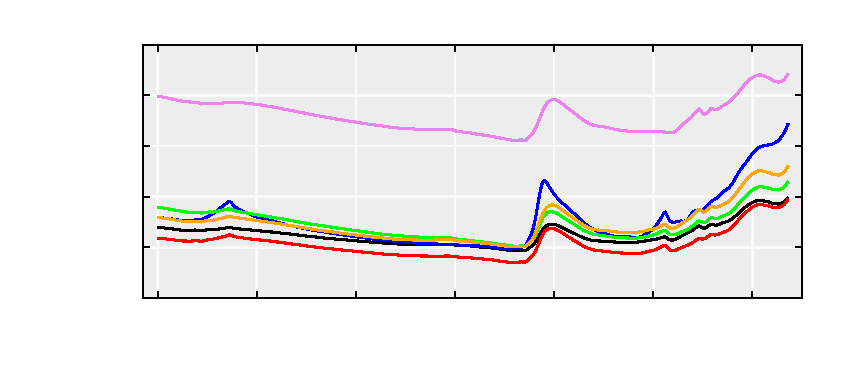
\includegraphics{gp/soil-spec-rnd}}%
    \gplfronttext
  \end{picture}%
\endgroup

			\caption{Six near infrared soil spectra of randomly chosen soil samples obtained from the data set, where $\lambda$ is the wavelength and $\rho(\lambda)$ the corresponding reflectance and each colour refers to one sample}
			\label{fig:soil-spec-rnd}
		\end{figure*}
		
	
	% subsection measured-data

	\subsection{Statistical Model}
	\label{ssec:statistical-model}
	
	
	

	
	% subsection statistical-model

	\subsection{Modellwahl im klassischen linearen Modell}
	\label{ssec:mlr}
	Im klassischen linearen Modell wird meist ... (s. Skript, S. XY)
	Das Problem mit der Wahl von $\alpha$ ...
	Beim Hinzufügen neuer Einflussgrößen in das Modell wird die Nullhypothese $H_0$ ...
	
		

	% subsection mlr

	\subsection{Mallow's $C_{p}$}
	\label{ssec:mallows-C_p}
	
		At this point, the model is specified using $k+1 = 320$ predictors for each response variable, using the whole domain of measured spectrum for each soil sample.
		
		
	
	
	% subsection mallows-C_p

	\subsection{Simulated Annealing}
	\label{ssec:model-selec}
	
		We can 

	% subsection simulated-annealing
		
	\subsection{Model Validation}
	\label{ssec:model-validation}
	
	
	% subsection model-validation
	
	\subsection{Assessment by Simulation}
	\label{ssec:simulation}
	
		
		
	% subsection simulation
% section methodology